\chapter{Methodology}
\label{chapter:methods}

The research was a qualitative study which followed design science research. This chapter introduces the methodology and methods as well as tools used in the study. Finally, the research implementation is presented.

\section{Design Science Research Methodology}
\label{section:overview}

\textcite{Aken:2014} describes \emph{Design Science Research DSR} to be a problem solving research strategy which should produce actionable knowledge in order to address types of field problems. The knowledge is used as a means, not as an end which means that the knowledge can be applied in a direct way to realize the desired outcomes. This is done by developing artefacts which should solve the problem experienced by people \parencite{Johannesson:2014}. As stated above, the design science research is driven by the field problems rather than knowledge problems, meaning that the problem is defined in the real world situation by stakeholders. 

According to \textcite{Johannesson:2014} the designed artefact can be a construct, method, model or instantiation. Constructs help to formulate problems and answers for them, meaning that they are definitional knowledge. Definitional knowledge means that with them it is possible to speak statements about the world rather than make the statements about the world. Methods define guidelines and processes which are meant to solve problems and achieve goals. Additionally, methods can be informal and be used as best practices. Models are used to represent possible solutions for a practical problem which means that they can be used to define the construction of the artefact. Lastly, instantiations are systems which are used in practice.

The design science research aims to produce a solution concept which would then be used to solve the field problem. This solution concept is used in the context by a design proposition. Design proposition can be formulated using CIMO-logic, which stands for this problem-in-\emph{C}ontext, it is useful to use this \emph{I}ntervention to produce through these \emph{M}echanisms this \emph{O}utcomes.

DSR-project has three parts \begin{enumerate}
\item An explanatory part which consist of analyzing and framing of the chosen type of field problem.
\item A design part when an intervention is designed and tested in an iterative way.
\item A testing part where the final version of the intervention is tested. \parencite{Aken:2014}
\end{enumerate}

\textcite{Peffers:2007} created a methodological framework for doing design science which complements and gives more precise activities for doing a DSR-project. This methodological framework, \emph{design science research methodology}, is divided into six different phases. The first activity is \emph{problem identification and motivation} where the specific research problem and justification of the value of a solution is defined. \emph{Defining the objectives for a solution} is the second activity where the objectives of a solution are inferred from the problem definition.

Next, the artifact which can be model, method, instantiation or construct is \emph{designed and developed}. Then the artifact is used to \emph{demonstrate} how it can be used to solve the identified problem. The artifact is \emph{evaluated} on how well it supports solving the research problem. This is done by comparing the objectives of a solution to the actual observed and measured results from the demonstration. Finally, the knowledge should be communicated to researchers.

\textcite{Salvatore:1995} state that design science aims to create things to serve human purposes. As stated earlier, the four types of products that design science aims to produce are constructs, models, methods and implementations. Additionally, design scientists develop ways to perform goal-directed activities which are innovative and valuable. The purpose of this study is to increase the understanding about housing company decision making as well as improve the current sales process. Thus, it is justified to use design science research since, as mentioned, the purpose of design science is to produce actionable knowledge to address the identified problems.

\section{Semi-structured Thematic Interview}
\label{section:interview-info}

According to \textcite{Wilson:2013} a semi-structured interview combines open-ended exploration with predefined questions and it usually follows a interview guide which offers a frame to conduct such interviews. The interview guide consists of an introduction to the topic and the purpose of the interview, a list of topics and predefined questions to ask, probs and promts and comments to end the interview.

The semi-structured interviews are done in a conversational manner even though there can be predetermined questions. It is a good method in order to investigate behaviours, opinions and emotions as well as to gather experiences. It provides a way to get more details about a topic where there is already some knowledge, but it lacks a deeper understanding. For the interviewee the semi-structured interview allows to focus on topics which they feel more important. In addition compared to the structured interview, the answers are open and not yes or no type of answers. \parencite{Cliffod:2010,Wilson:2013}

According to \textcite{HH:2001} semi-structured thematic interview is based on the focused interview which was published in a book \emph{The Focused Interview} written by Merton, Fiske and Kendall. The most relevant aspect of thematic interview is that the interview is going forward based on the themes rather than detailed questions so, it provides a framework for discussion. This allows the interviewees to answer more freely with their own wordings in order to bring their experiences to the center of attention and thus for the interviewer it is possible to collect insights about what people do and think \parencite{Cliffod:2010}.

As stated above, semi-structured interview as well as thematic interview have many strengths considering the flexibility, gathering experiences and the comparison between the interviews. However, it is important to be aware of that the interviewer do not put words into the interviewee's mouth or guide the discussion into particular answer during the interview. Since, the semi-structured interview is flexible, it is crucial for the interviewer to be also consistent in order to make comparisons between the interviews. \parencite{Wilson:2013}

Since, the purpose of first research question was to find out what affects the purchasing decision making in the housing board it was justified to conduct semi-structured thematic interviews in order to discover the real feelings and operations inside the board. The interview was chosen because it provides a way to get deeper understanding by collecting detailed information \parencite{Johannesson:2014}. In addition the semi-structured interview allows the discussion to flow freely and the interviewees were able to describe the situations more broadly compared to structured interview.

\section{Lean Service Creation}

It is stated by \textcite{LSC} that \emph{Lean Service Creation LSC} helps bringing customer centricity into work, workflow and internal process development. Additionally, the LSC helps to communicate ideas and it forms a shared language. In practice, LSC is a set of tools which help multidisciplinary teams to create new services and products. It is based on Lean Startup, Agile methods and Design thinking. LSC offers canvases which outline the relevant phases in a service creation process and it is at the hands of the user to decide in which order the canvases should be used. According to the creators of LSC, the mindset and practices are the foundation for successful service creation.

Since, the actual study was conducted as a service design project it was justified to use some tool set which would help the research process. Lean Service Creation was chosen because it was familiar for the researcher and it also fit the process of the design science research. Moreover, LSC helps to think more about the customers and thus, the usage will increase the customer centricity. 


\section{Research Implementation}
\label{section:research-implementation}

The Next chapters describes how the actual research was done phase by phase. The phases of the design science research methodology together with activities done during the study are presented in the The Figure~\ref{fig:dsrm-implementation}.

\begin{figure}[ht]
  \begin{center}
    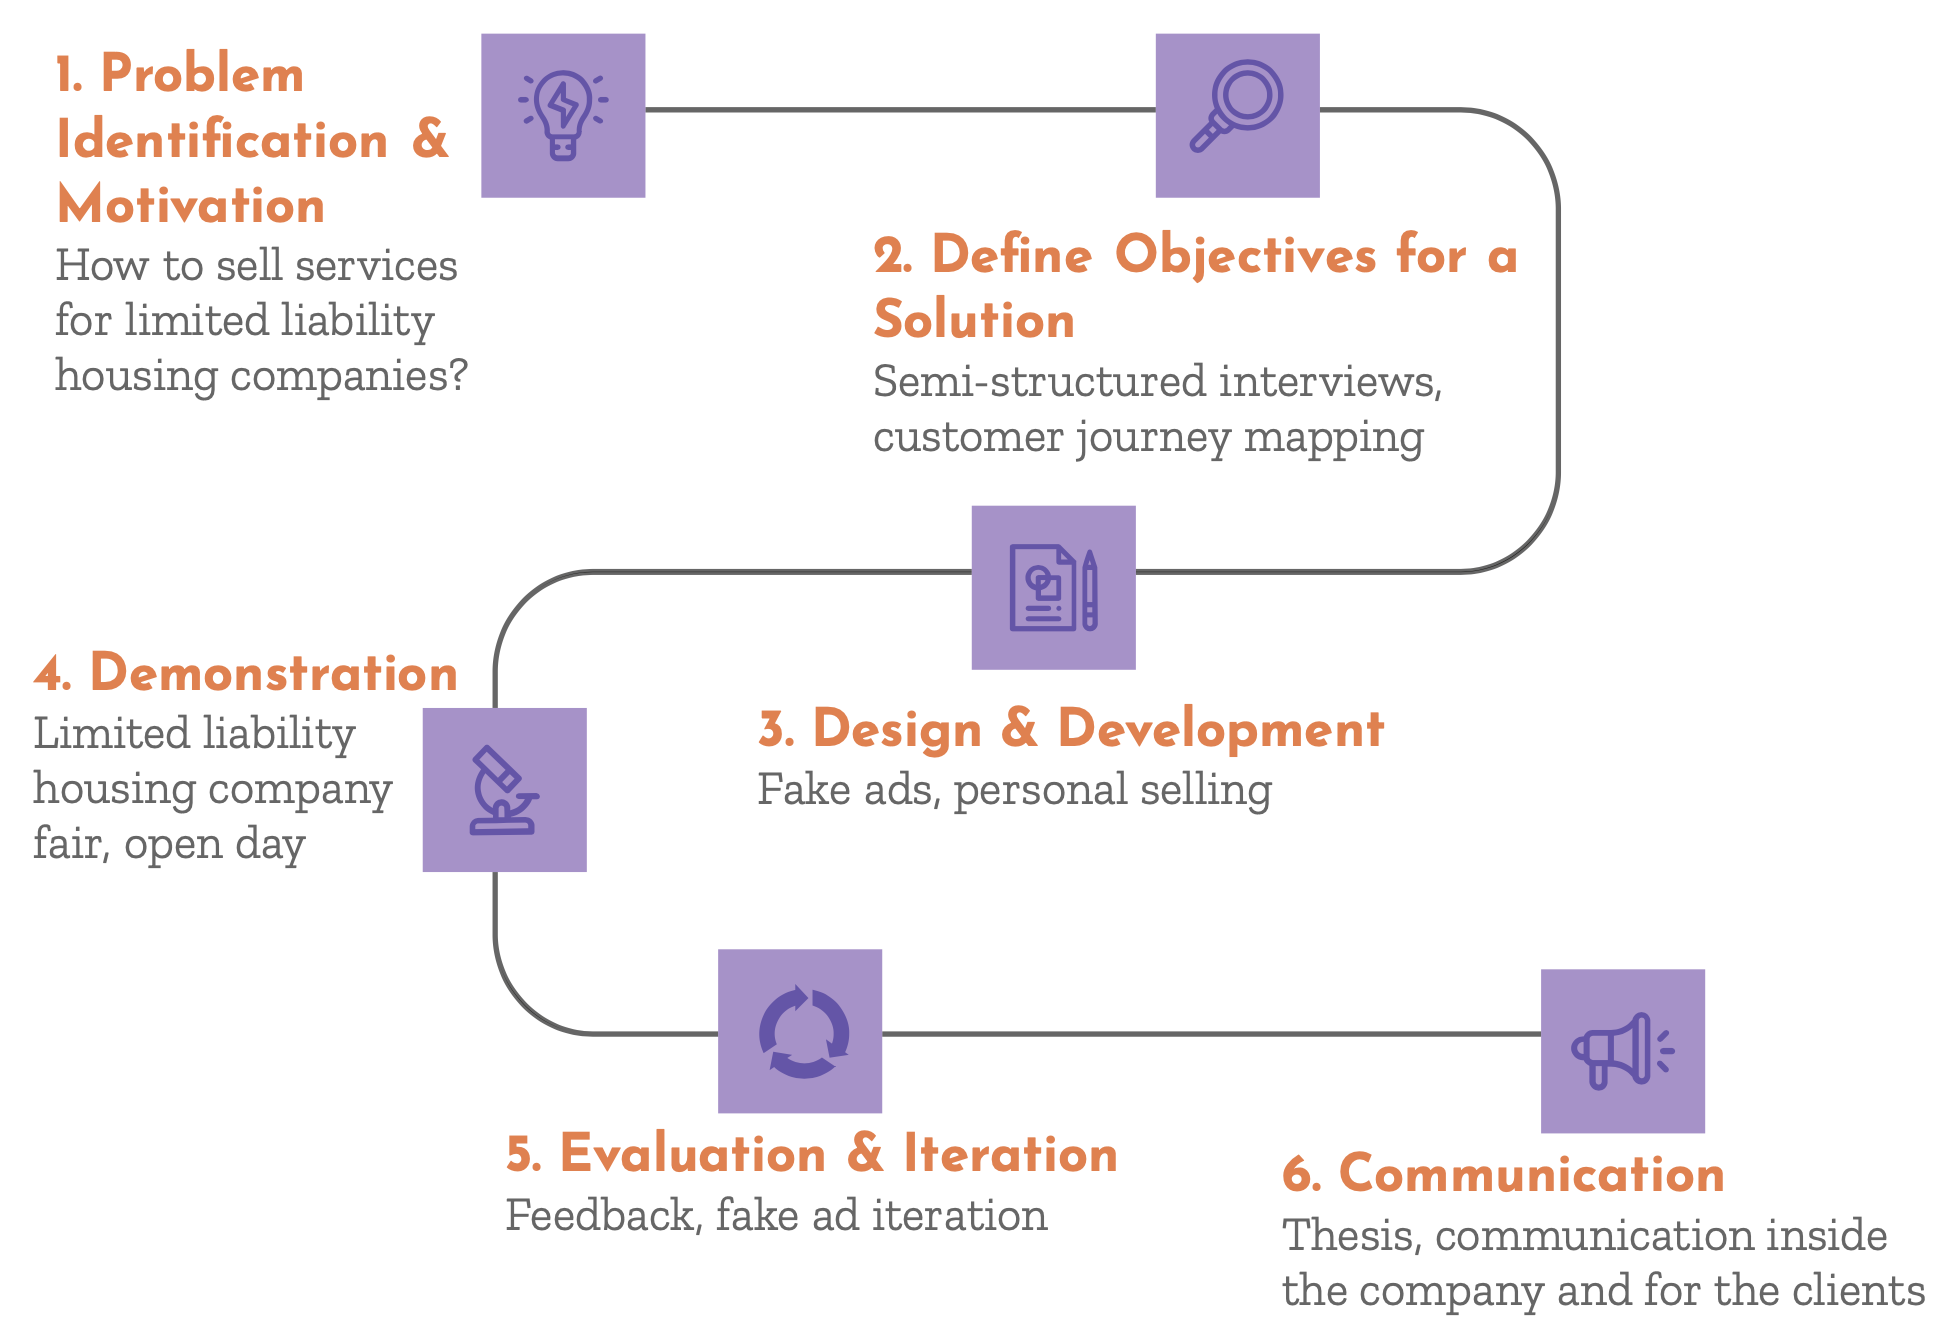
\includegraphics[width=\textwidth]{dippa/images/dsrm-implementation.png}
    \caption{The research process and the conducted activities.}
    \label{fig:dsrm-implementation}
  \end{center}
\end{figure}

\subsection{Activity 1: Problem Identification and Motivation}

Based on the DSRM process the study started with the first activity, problem identification and motivation. The case company was in the situation where they needed to expand their sales, and in order to grow bigger in Finland, they needed housing companies as clients. The problem in acquiring them as clients was that the case company had not done business to customer selling much and they needed to gain more understanding about how the housing company works and makes decisions. This problem then lead to the first research question \emph{What affects the purchase decision making in a limited liability housing companies}.

In addition to understanding the decision making in housing companies, it was important to discover a sales process which would take into account the case company's and partners viewpoints as well as the end-customers' viewpoints in order to make acquiring housing companies as clients easier, faster and unified. From this problem the second research question was formed as \emph{How to improve current sales process with the knowledge of limited liability housing company’s decision making process?}

Literature review was conducted in the Chapter 2 and it included the relevant background research about housing company, energy industry in Finland, decision making process and customer centricity. housing companies were studied in order to understand the operation and the legal backgrounds of its actions. Energy industry in Finland were researched in order to understand the current state and future opportunities. In order to design some improvements for the sales process it was crucial to understand how humans make purchasing decisions. Lastly, the concept and benefits of customer centricity was presented.

In order to understand the motivation and the problems of energy companies, the researcher participated in several partner meetings and observed them. In addition the researcher did observation at the workplace and that knowledge was applied in several occasions. The researcher also used few canvases from the LSC in order to make communication easier with the relevant stakeholders and to make the discussed topics more tangible.

\subsection{Activity 2: Defining Objectives for a Solution}

\subsubsection*{Data Gathering}

The second activity of a DSRM, defining objectives for a solution was done by conducting semi-structured interviews with the board members of housing companies. To gain broader understanding the researcher did six interviews with people of different age and their experience level in the board varied from one year to almost twenty years. Additionally, the people were either chairpersons or members of the board. The interviews that lasted from 40 to 80 minutes and they were conducted as face to face meetings and recorded in order to listen and analyze them afterwards. The relevant information related to the interviewees role, experience in the board, age, occupation and the duration of the interviews are presented in the Table~\ref{table:interviewtb}.

The thematic interview was divided into four categories in order to answer the \emph{RQ1: What affects the purchase decision making in a private housing company board}. These themes were defined in order to gain insights about why people go to board, how the board operates in practice and what kind of things influence their work. The themes covered in the interviews were as follow: being part of the board, decision making in the board, influences on housing company operations and energy efficiency. The first theme dealt with reasons why the interviewees were members of the board and their feelings about their work in the board in general. Second theme covered the process of decision making with examples of previously made investment decisions and the role of money in them. Third theme concentrated to learn about influences that affects the operations of the board as well as who the board trust and where they find information related to services provided for housing companies. Lastly the energy efficiency topic discovered how well are energy efficiency topics understood in the boards of the housing companies and the importance of it.

\begin{table}
\begin{tabular}{|p{2.3cm}|p{2.8cm}|p{1.8cm}|p{2.7cm}|p{1.9cm}|} 
% Alignment of sells: l=left, c=center, r=right. 
% If you want wrapping lines, use p{width} exact cell widths.
% If you want vertical lines between columns, write | above between the letters
% Horizontal lines are generated with the \hline command:
\hline % The line on top of the table
\textbf{Role} & \raggedright\textbf{Experience in the board} & \textbf{Age} & \textbf{Occupation} & \textbf{Duration} \\ 
\hline 
% Place a & between the columns
% In the end of the line, use two backslashes \\ to break the line,
% then place a \hline to make a horizontal line below the row 
Member & 17 years & 59 years & Director & 40 mins \\ 
\hline
Member & 11 years & 36 years & Energy expert & 80 mins \\  
\hline
Chairperson & 5 years & 30 years & IT-consultant & 80 mins \\
\hline
Chairperson & 10 years & 76 years & retired & 60 mins \\
\hline
Chairperson & 19 years & 70 years & retired & 75 mins \\
\hline
Chairperson & 1 year & 31 years & Electronics engineer & 45 mins \\
\hline
\end{tabular} % for really simple tables, you can just use tabular
% You can place the caption either below (like here) or above the table
\caption{Information about the interviewees.}
% Place the label just after the caption to make the link work
\label{table:interviewtb}
\end{table} % table makes a floating object with a title

\subsubsection*{Data Analysis of the Interviews}

\textbf{Analyzing of the interviews was done by listening the interviews again and taking notes of relevant points and afterwards clustering them into categories.} The researcher divided the notes based on the LSC user insight canvas since it was familiar way for the researcher to help analyzing the interviews. The user insight canvas categorizes the notes for user needs and problems, what surprised the researcher and what the user thinks and feels.

According to \textcite{HH:2001} the researcher knows the interview material so well that it is easy for her to recognize the themes covered and make notes about dialogue when needed. Thus, in this study the researcher did not transcribe the interviews since there were only six interviews to be analyzed and the researched conducted the interviews alone.

\subsubsection*{Observing the Energy Industry}

\textbf{In addition to the interviews}, the researcher participated many meetings where the energy company was present in order to \textbf{observe} and gain more insights about the industry. From the meetings, the researcher gained understanding on how well do the energy companies understand the housing companies as their customers and how much they have communication with them. Additionally, the researcher learned about the drivers to have case company's solution as part of the company's service offering. To understand more about the energy company the researcher and the team categorized energy companies into three different segments based on their team size, speed to take things forward and willingness to proceed with service business.

\subsubsection*{Customer Journey Mapping}

To design a better way and providing guidance on how to acquire customers it was first necessary to go through the current customer journey as described in the chapter 2.4.1. For this, the researcher used LSC canvas for visualizing customer engagement. The canvas helps to list all the steps from rising customer awareness, engagement, purchase, use, use more and advocate combined with the touchpoints. By listing also the enablers and problems it was easier to discover problems.

The canvas was filled with one energy company and it was also complemented with the knowledge gained from other meetings with energy companies. From this work it was decided to focus on the first three steps in customer engagement canvas which were awareness, engagement and purchase because it was identified that those are the biggest bottlenecks. Additionally the case company's product is sold by the partners and they can sell the service in which form the want but they lack the knowledge about how to actually approach the housing companies.

\subsection{Activity 3: Design and Develop}

The third activity in design science research is design and develop and the purpose is to design an artefact which addresses the stated problem and fulfills the defined objectives \parencite{Johannesson:2014}. So, to answer the second research question \emph{How to improve current sales process with the knowledge of limited liability housing company’s decision making process?} the researcher together with the team conducted few tests to gain insights which would then work as a base for improvement suggestions. The Figure~\ref{fig:experiments} presents the two tests which were done related to the pricing model and personal selling as well as consulting.

\begin{figure}[ht]
  \begin{center}
    % here the width of the figure is set to 9 cm
    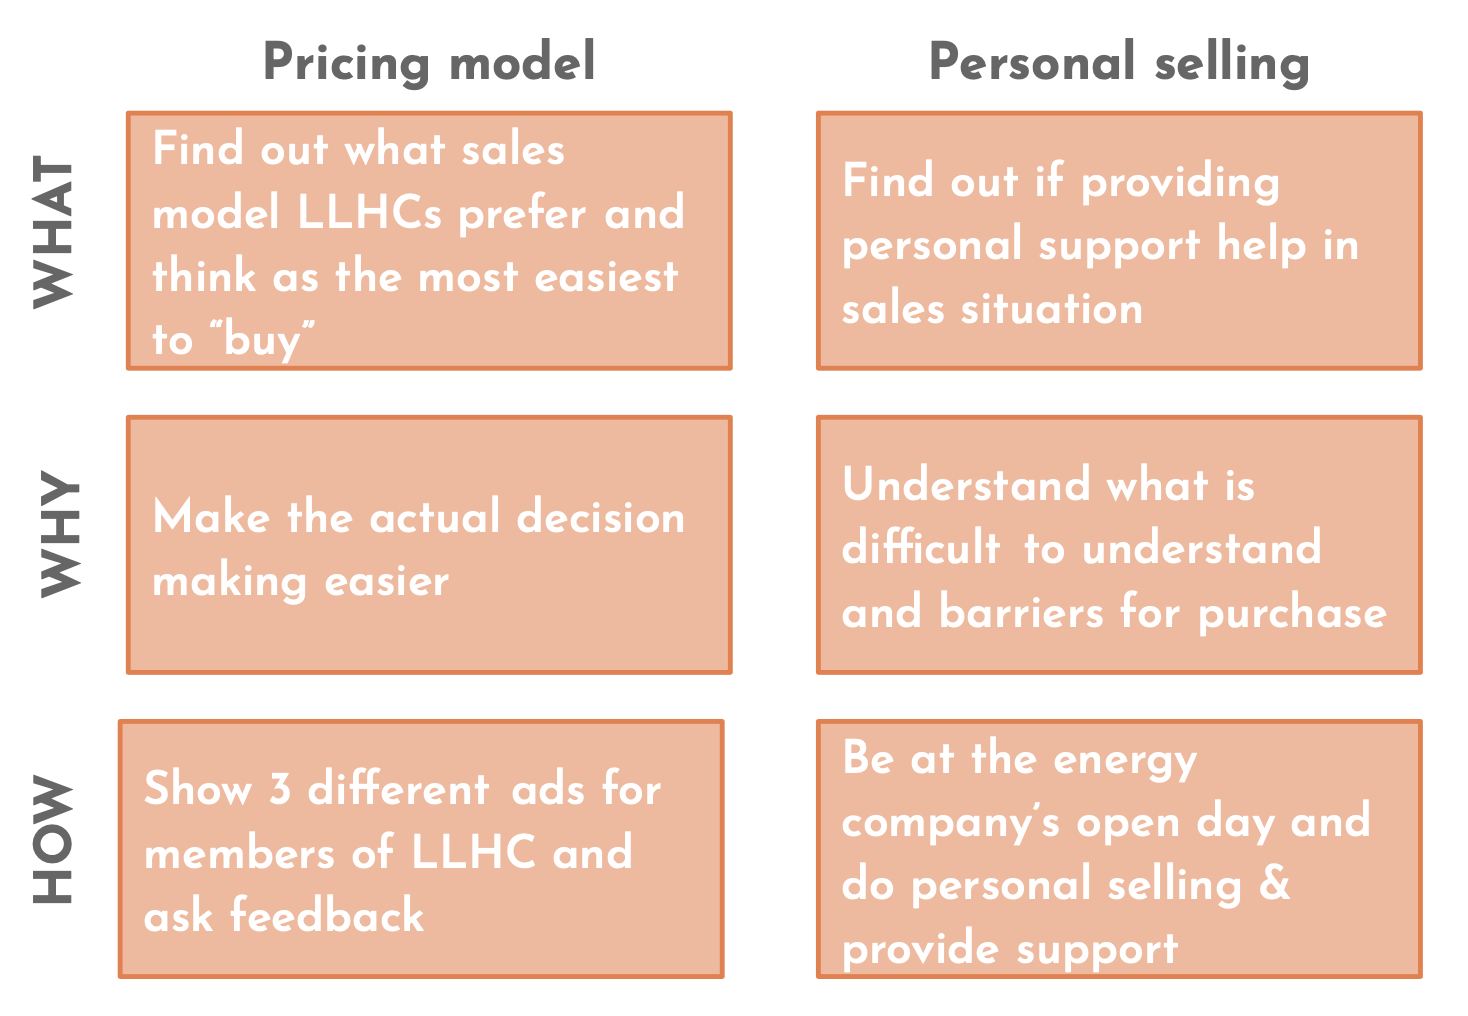
\includegraphics[width=\textwidth]{dippa/images/experiments.png}
    \caption{Conducted experiments.}
    \label{fig:experiments}
  \end{center}
\end{figure}

\subsubsection*{Fake Ads}

Pricing model had risen as a big concern among the case company and the energy companies since they did not know what model would work best for the housing company. In addition, the partner company had a service already in the market but they were struggling with the pricing model. So, to find out which model the housing boards would prefer and why, the researcher and the team designed three different fake ads which were all looking the same but the pricing model was different in each of the ads. Additionally, the communication of the fake ads were following the \emph{start with why} philosophy as described previously in the chapter 2.3.

The fake ads had three different kinds of pricing models which were as follows:
\begin{itemize}
	% You can use this command to set the items in the list closer to each other
	% (ITEM SEParation, the vertical space between the list items) 
	\setlength{\itemsep}{2pt}
	\item Investment plus a monthly service fee,
	\item A monthly service fee.
	\item A monthly service fee which is covered by the saved energy fees.
\end{itemize}

\subsubsection*{Personal Selling with Personalized Offers}

From the interviews done with the housing companies, it was clear that they need consulting and help when the offered service is new to them. Additionally, clear communication, making things as simple as possible and providing support are important when being in contact with them. With this in mind the the researcher participated one open day organized by an energy company in Finland. There the researcher was able to provide support and answer the questions about the service. Moreover the researcher was able to do personal selling. Lastly, to improve the engagement and to help purchase decision making easier the researcher and the team made personalized offers, which were available in the open day, by adding the potential amount of saving for the housing companies. This was done in order to reduce the pain and increase the net value as presented in the chapter 2.3.

\subsection{Activity 4: Demonstrate}

\subsubsection*{Limited Liability Housing Company Fair}
The three different fake ads designed were tested in the housing company fair which was aimed for the board members of housing companies. The specific fair was chosen because the main audience there were purely the board members because the idea behind the fair is to present services and products for the housing companies. The fake ad testing was done together with one energy company who is also partner of the case company.

The ads were shown for 12 people and asked to read and comment the ads. The testing was done mainly in pairs which allowed the other to present the ads and the other to make notes about the test session. The team approached people in the fair and asked if they would be willing to give opinions about the ads. The ads were given for the volunteers and after a moment the people needed to choose one of the ads which had the pricing model that they prefer the most. The team asked reasons behind the choice and also feedback about the ads in order to find out improvement ideas.

\subsubsection*{Energy Company's Open Day}

Since, it was clear from the interviews that lack of expertise in real estate or building industry are typical issues in housing companies the researcher took part in an energy company's open day in eastern Finland in order to do personal selling. The purpose was to be there in person and to promote their service which is built on top of the case company's technology. In the open day the researcher had personalized offers for the area's housing companies.  The offers also included improvements from the previous test done in the housing company fair.

The offers all had the same monthly cost but in the offer it was also stated how much is the predicted saving if they would have the service in use. The researcher was able to contact the members of housing companies in person, answer the questions immediately and also to collect contact information from interested buyers.

The researcher was able to discuss with three members of housing company, the rest of the people were mainly living in detached houses. All of them received an offer and their contact information was collected for the energy company to be in contact with them afterwards.

\subsection{Activity 5: Evaluate and Iterate}

In the second to last activity of DSRM the designed artefact is evaluated to see how well it solve the initial problem and fulfil the set requirements. To answer the RQ1 the researcher analyzed the interviews and formed requirements which were then used to form guidance of how the improved sales process should go. Additionally, the interview result can be used as guidance since they increase the understanding of the operation of housing company.

To answer the RQ2, the researcher together with team did different test to gain insights about what works and what not in acquiring housing companies as clients. The test were evaluated also from the business perspective and objectives.

Since, the purpose of this study was to gain more knowledge about the housing companies and to form suggestions the results can also be used in order to find out future research areas.

Iteration was not possible to do for the whole process because of the research time span. However, the ads were improved after test sessions and the insights gained from the test sessions were always further used in the next sessions as well as daily work. In addition, the researcher describe the future research ares and recommendations of what should be done next.

\subsection{Activity 6: Communicate}

The last activity of the DSRM consist of communicating the results of the study and this is done through this thesis. In addition, the results are presented in the case company as well as for the case company's energy company partners if possible.